% This template was written by Benoît Legat and is inspired from https://fr.overleaf.com/latex/examples/quadratic-function/hjbvztxdrvwf

% 2 COLUMNS

\documentclass[final]{beamer}

\usepackage[scale=1.24]{beamerposter}
\usetheme{ICTEAMposter} % `ICTEAMposter` theme of `beamerposter` package

%-----------------------------------------------------------
% Define the column widths and overall poster size
% To set effective sepwid, onecolwid and twocolwid values, first choose how many columns you want and how much separation you want between columns
% In this template, the separation width chosen is 0.024 of the paper width and a 4-column layout
% onecolwid should therefore be (1-(# of columns+1)*sepwid)/# of columns e.g. (1-(4+1)*0.024)/4 = 0.22
% Set twocolwid to be (2*onecolwid)+sepwid = 0.464
% Set threecolwid to be (3*onecolwid)+2*sepwid = 0.708
\newlength{\sepwid}
\newlength{\onecolwid}
\newlength{\twocolwid}
\newlength{\threecolwid}
\setlength{\paperwidth}{36.0in} % A0 width: 46.8in (default: 36in)
\setlength{\paperheight}{48.0in} % A0 height: 33.1in (default: 48in)
\setlength{\sepwid}{0.024\paperwidth} % Separation width (white space) between columns
\setlength{\onecolwid}{0.464\paperwidth} % Width of one column
%\setlength{\twocolwid}{0.464\paperwidth} % Width of two columns
\setlength{\threecolwid}{5\paperwidth} % Width of three columns
\setlength{\topmargin}{-0.5in} % Reduce the top margin size
%-----------------------------------------------------------

%\linepenalty=5000

\usepackage{booktabs} % Top and bottom rules for tables
%\usepackage[load-configurations = abbreviations]{siunitx}

\usepackage[backend=bibtex]{biblatex}
\bibliography{biblio.bib}
\renewcommand*{\bibfont}{\footnotesize }
\definecolor{myGreen}{RGB}{168, 178, 85}
\usepackage{bbm}
\DeclareMathOperator{\Tr}{Tr}
\DeclareMathOperator*{\argmax}{arg\,max}
\usepackage{adjustbox}
\usepackage[para]{threeparttable}
\usepackage{multirow}
\usepackage{tabularx}
\usepackage{textcomp}
\usepackage{graphicx}
%\usepackage{subcaption}
\usepackage{textpos}
\usepackage{svg}
%\setbeamerfont{enumerate item}{size=\large}

\tolerance=2000
%\emergencystretch=\maxdimen
\emergencystretch=15pt
\hyphenpenalty=9500
\hbadness=9500

\newcommand{\placetextbox}[4][center]{%
  % [#1]: box anchor: center (default) | 
  %                 south west | west | north west | north |
  %                 north east | east | south east | south | 
  %                 mid west | mid | mid east |
  %                 base west | base | base east 
  % #2: horizontal position (fraction of page width)
  % #3: vertical position (fraction of page height)
  % #4: content
  %
  \tikz[remember picture,overlay,x=\paperwidth,y=\paperheight]{%
    \node[anchor=#1,inner sep=0pt]
    at ($(current page.south west)+(#2,#3)$) {#4};
  }%
}

\title{Hardware Acceleration on FPGA of an Integrated \\ Sensing and Communication OFDM Chain 
%for a Wi-Fi 6 USRP-based Experimental Setup
}

\author{\underline{Quentin Prieels} quentin.prieels@student.uclouvain.be}

\institute{Supervisors: Prof. Jérôme Louveaux and Prof. Martin Andraud - Assistants: Martin Willame and Pol Maistriaux}

%----------------------------------------------------------------------------------------

% https://tex.stackexchange.com/questions/426088/texlive-pretest-2018-beamer-and-subfig-collide
\makeatletter
\let\@@magyar@captionfix\relax
\makeatother

\begin{document}

\addtobeamertemplate{block end}{}{\vspace*{2ex}} % White space under blocks
\addtobeamertemplate{block alerted end}{}{\vspace*{2ex}} % White space under highlighted (alert) blocks

\setlength{\belowcaptionskip}{2ex} % White space under figures
\setlength\belowdisplayshortskip{2ex} % White space under equations

\begin{frame}[t,fragile] % The whole poster is enclosed in one beamer frame

%\placetextbox[center]{0.97}{0.87}{
\includegraphics[height=6cm]{I.png}}

\begin{columns}[t]% The whole poster consists of three major columns, the second of which is split into two columns twice - the [t] option aligns each column's content to the top

\begin{column}{\sepwid}\end{column} % Empty spacer column

%%%%%%%%%%%%%%%%%%%%%%%%%
% 1) The first column
%%%%%%%%%%%%%%%%%%%%%%%%%
\begin{column}{\onecolwid}
  
  \par\vskip\medskipamount
  \usebeamerfont{block body}
  \vskip0.178cm
  \justifying

  \vspace{-0.7cm}
  %\vspace{-0.5in}


  \begin{alertblock}{Abstract}
    Both communication and RADAR systems exploit the same frequency spectrum, but for different purposes. 
    The first aims to transmit unknown data, the second aims to detect targets and estimate their parameters, such as velocity or distance. 
    As they share processing steps, why not combine them in a single system? 
    How to achieve a sufficient level of performance to be able to process data in real-time?
  \end{alertblock}

  %\vspace{-0.2in}

  \begin{block}{Context}
    In recent years, the concept of integrated sensing and communication systems (ISAC) has gained attention. 
    \textbf{Combining data transmission and target detection} into a single system, would enable to: \vspace{-0.2in}
      \begin{itemize}
        \item \hspace{0.2cm} exploit the frequency spectrum more efficiently;
        \item \hspace{0.2cm} reduce the number of hardware needed.
        %\item \hspace{0.2cm} reduce the energy consumption.
      \end{itemize}
      %\newline

    From autonomous vehicles to health monitoring, ISAC systems have a wide range of applications. 
    Especially in the context of the Internet of Things (IoT) where billions of connected devices are already deployed and rely on wireless communication like Wi-Fi.\newline

    New standards, like the upcoming 802.11bf, are being defined to support sensing capabilities in Wi-Fi networks. 
    Based on \textbf{Orthogonal Frequency Division Multiplexing (OFDM) modulation}, Wi-Fi Sensing can be used to detect the presence of people, monitor their movements, or even perform fall detection.
  \end{block}

  %\vspace{-0.2in}

  \begin{block}{Experimental setup}
    Proof of concept of ISAC exists, with an \textbf{experimental setup} developed at UCLouvain. 
    %It performs basic communication and radar functions using signals defined by the Wi-Fi 6 standard. 
    Based on a software implementation using Software-Defined Radio (SDR), it first captures the received signal, then \textbf{process data offline}. 
    It uses the Universal Software Radio Peripheral (USRP) devices from Ettus Research to transmit and receive signals.

    \vspace{0.5in}

    \begin{figure}[!ht]
      \centering
      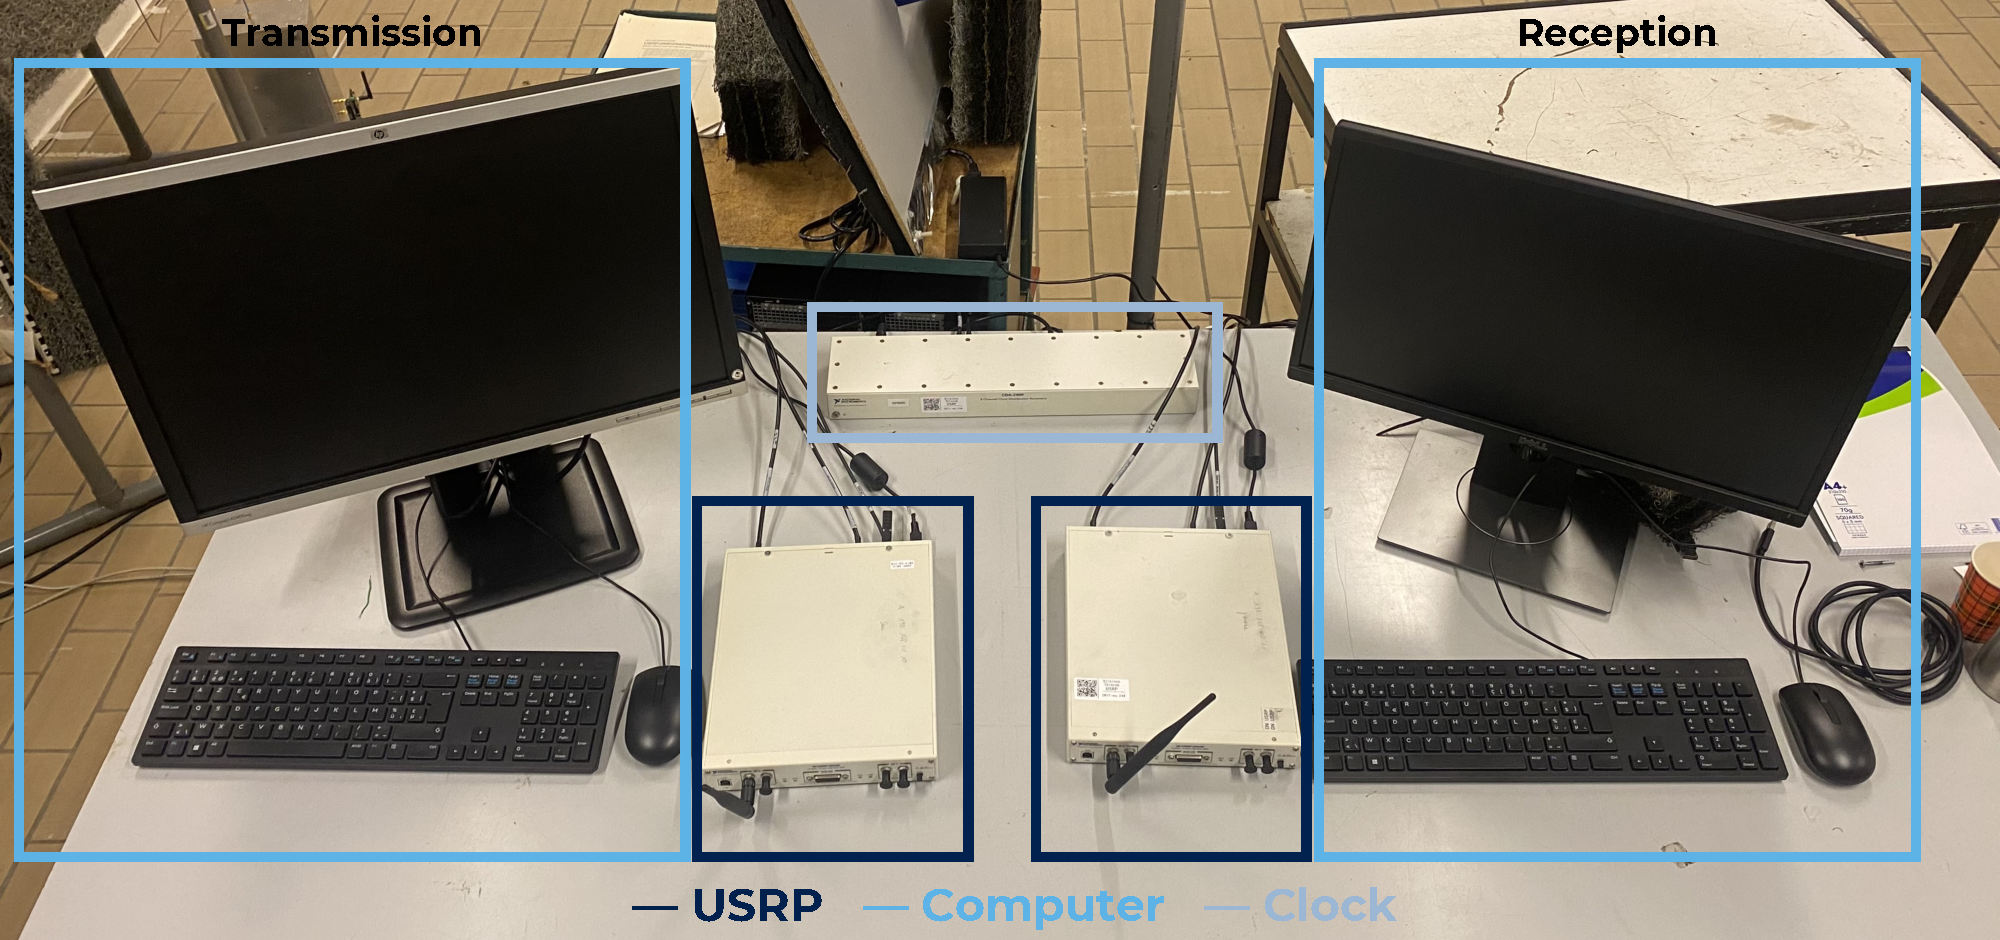
\includegraphics[width=\linewidth]{img/setup.pdf}
      \caption{USRP-based experimental setup}
    \end{figure}
  \end{block}

\end{column}

\begin{column}{\sepwid}\end{column} % Empty spacer column

%%%%%%%%%%%%%%%%%%%%%%%%%
% 2) The second column
%%%%%%%%%%%%%%%%%%%%%%%%%
\begin{column}{\onecolwid}

  %\vspace{-0.5in}

  \begin{block}{Objective}
    USRP devices embed \textbf{Field-Programmable Gate Arrays (FPGAs)} that can be programmed to accelerate the processing of the data. 
    By implementing several blocks of the OFDM receiver chain, like time synchronization or Fast Fourier Transform (FFT) on the FPGA, it is possible to speed up the processing and \textbf{target real-time data processing}.

    %\vspace{-0.1in}

    \begin{figure}[!ht]
      \centering
      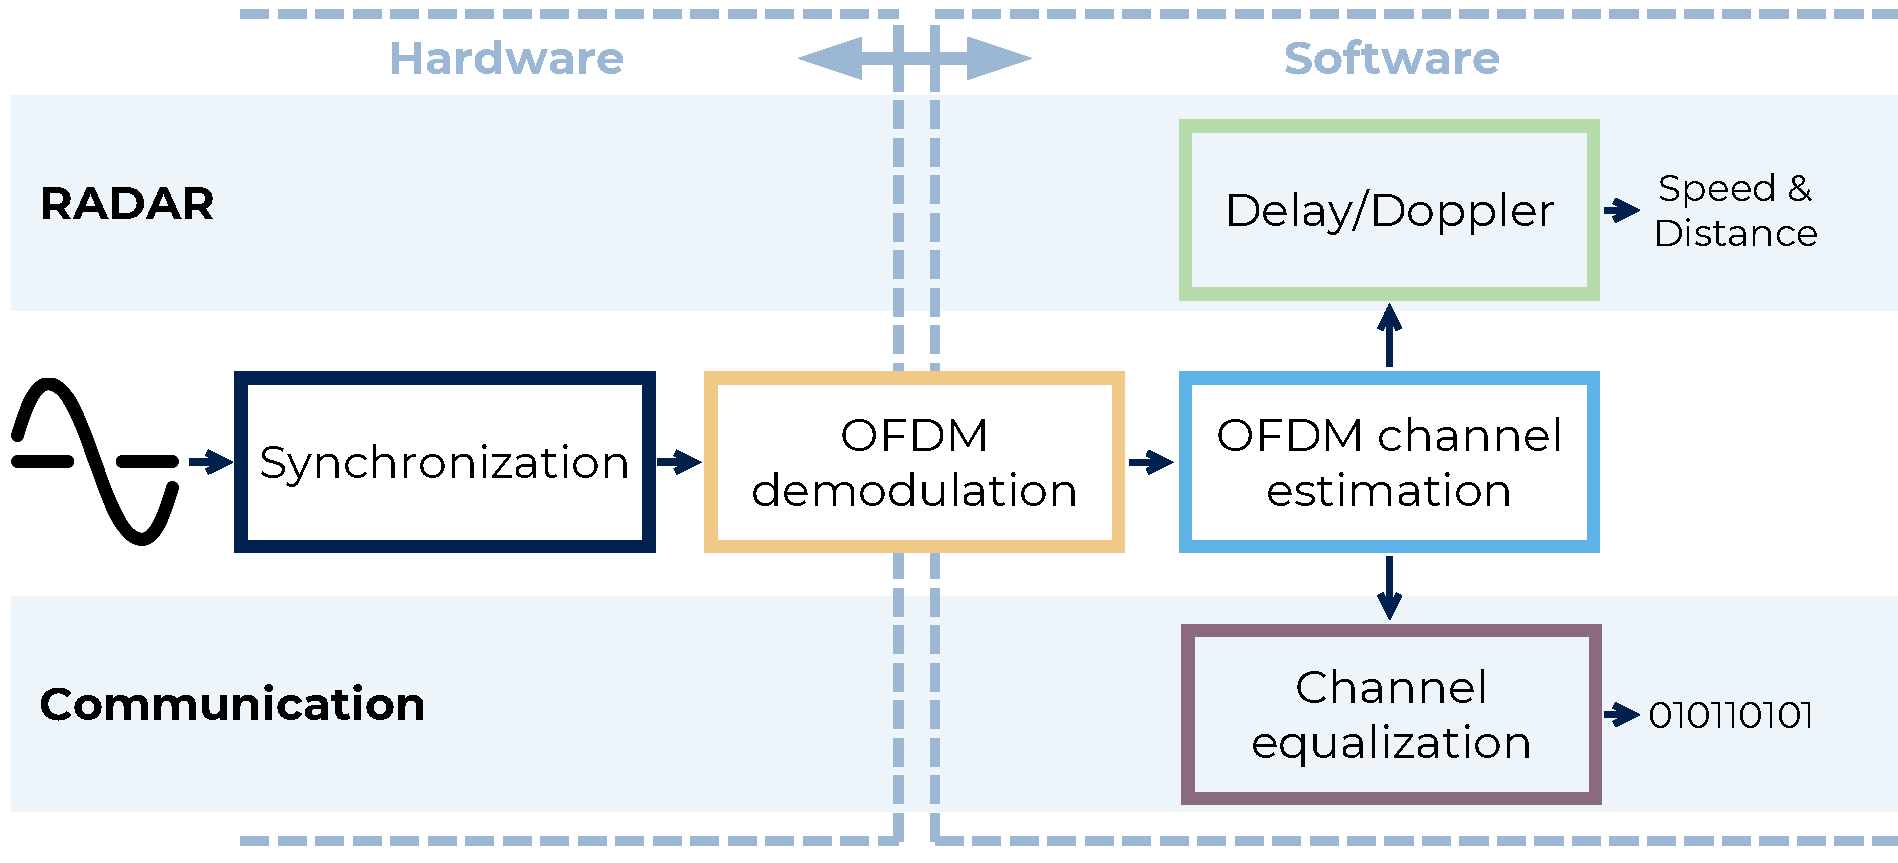
\includegraphics[width=\linewidth]{img/ofdm_reciever_chain_h.pdf}
      \caption{OFDM receiver chain}
    \end{figure}

    Some blocks of the processing pipeline take more time than others. Therefore, there are more interesting to accelerate.

    \vspace{0.2in}

    \begin{figure}[!ht]
      \centering
      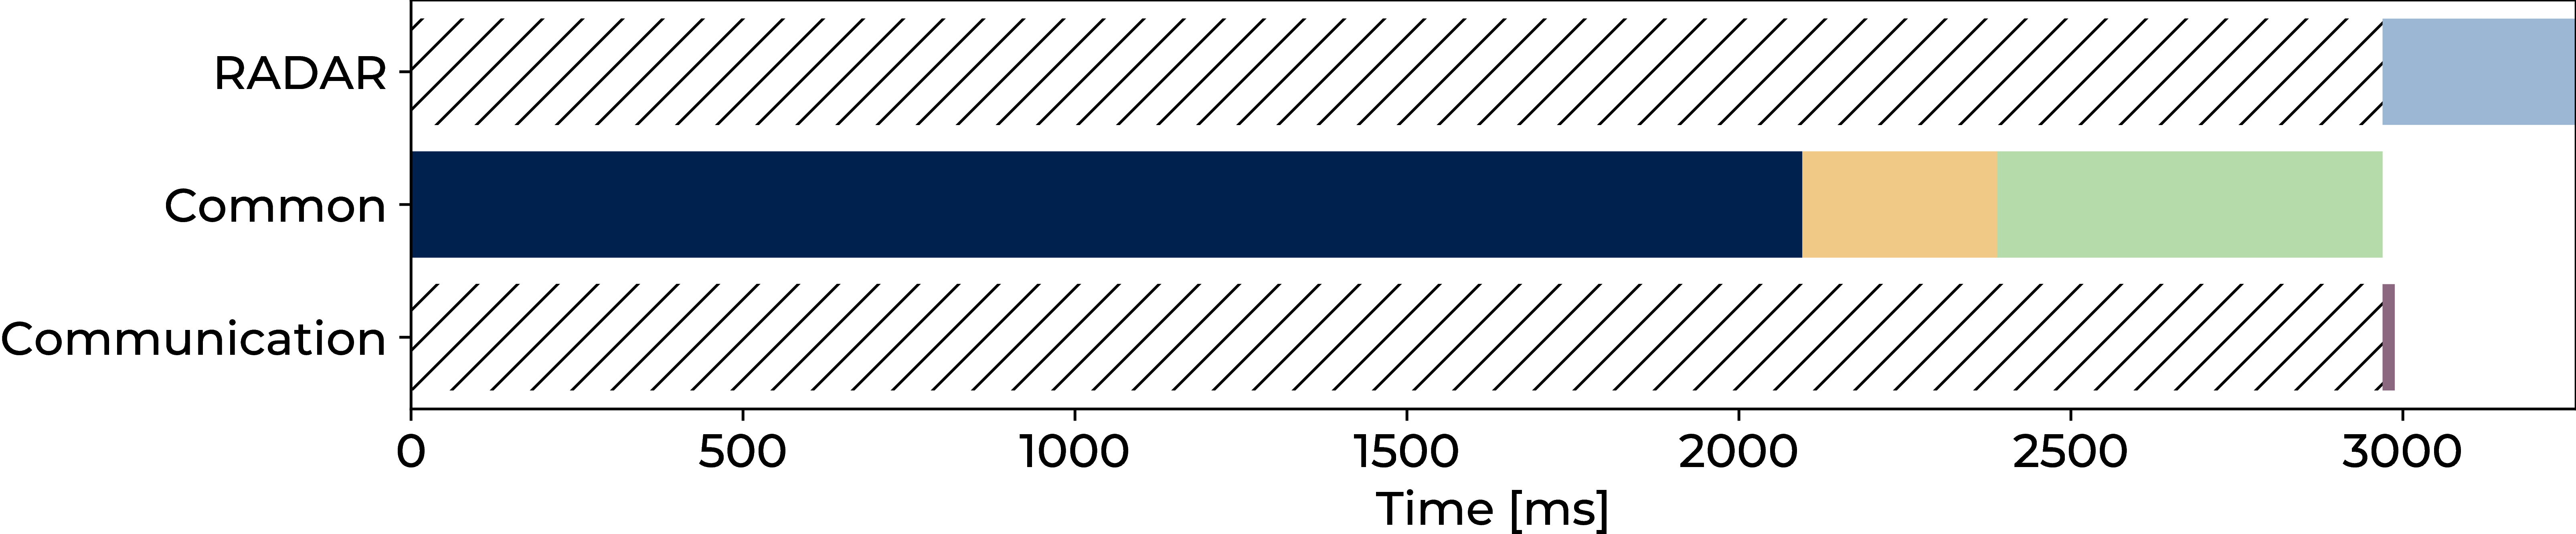
\includegraphics[width=\linewidth]{../../experiments/01/complexity.png}
      \caption{Time taken by each block of the receiver chain for a 2048 OFDM symbols packet}
    \end{figure}

  \end{block}

  %\vspace{-0.8in}

  \begin{block}{Approach}
    Internally, the FPGA of the USRP devices is composed of several blocks that can be interconnected to create a custom processing chain. 
    Ettus Research developed the \textbf{RFNoC} (RF Network on Chip) framework to facilitate the development of FPGA-based signal processing chains and enable the integration of custom processing blocks.

    \begin{figure}[!ht]
      \centering
      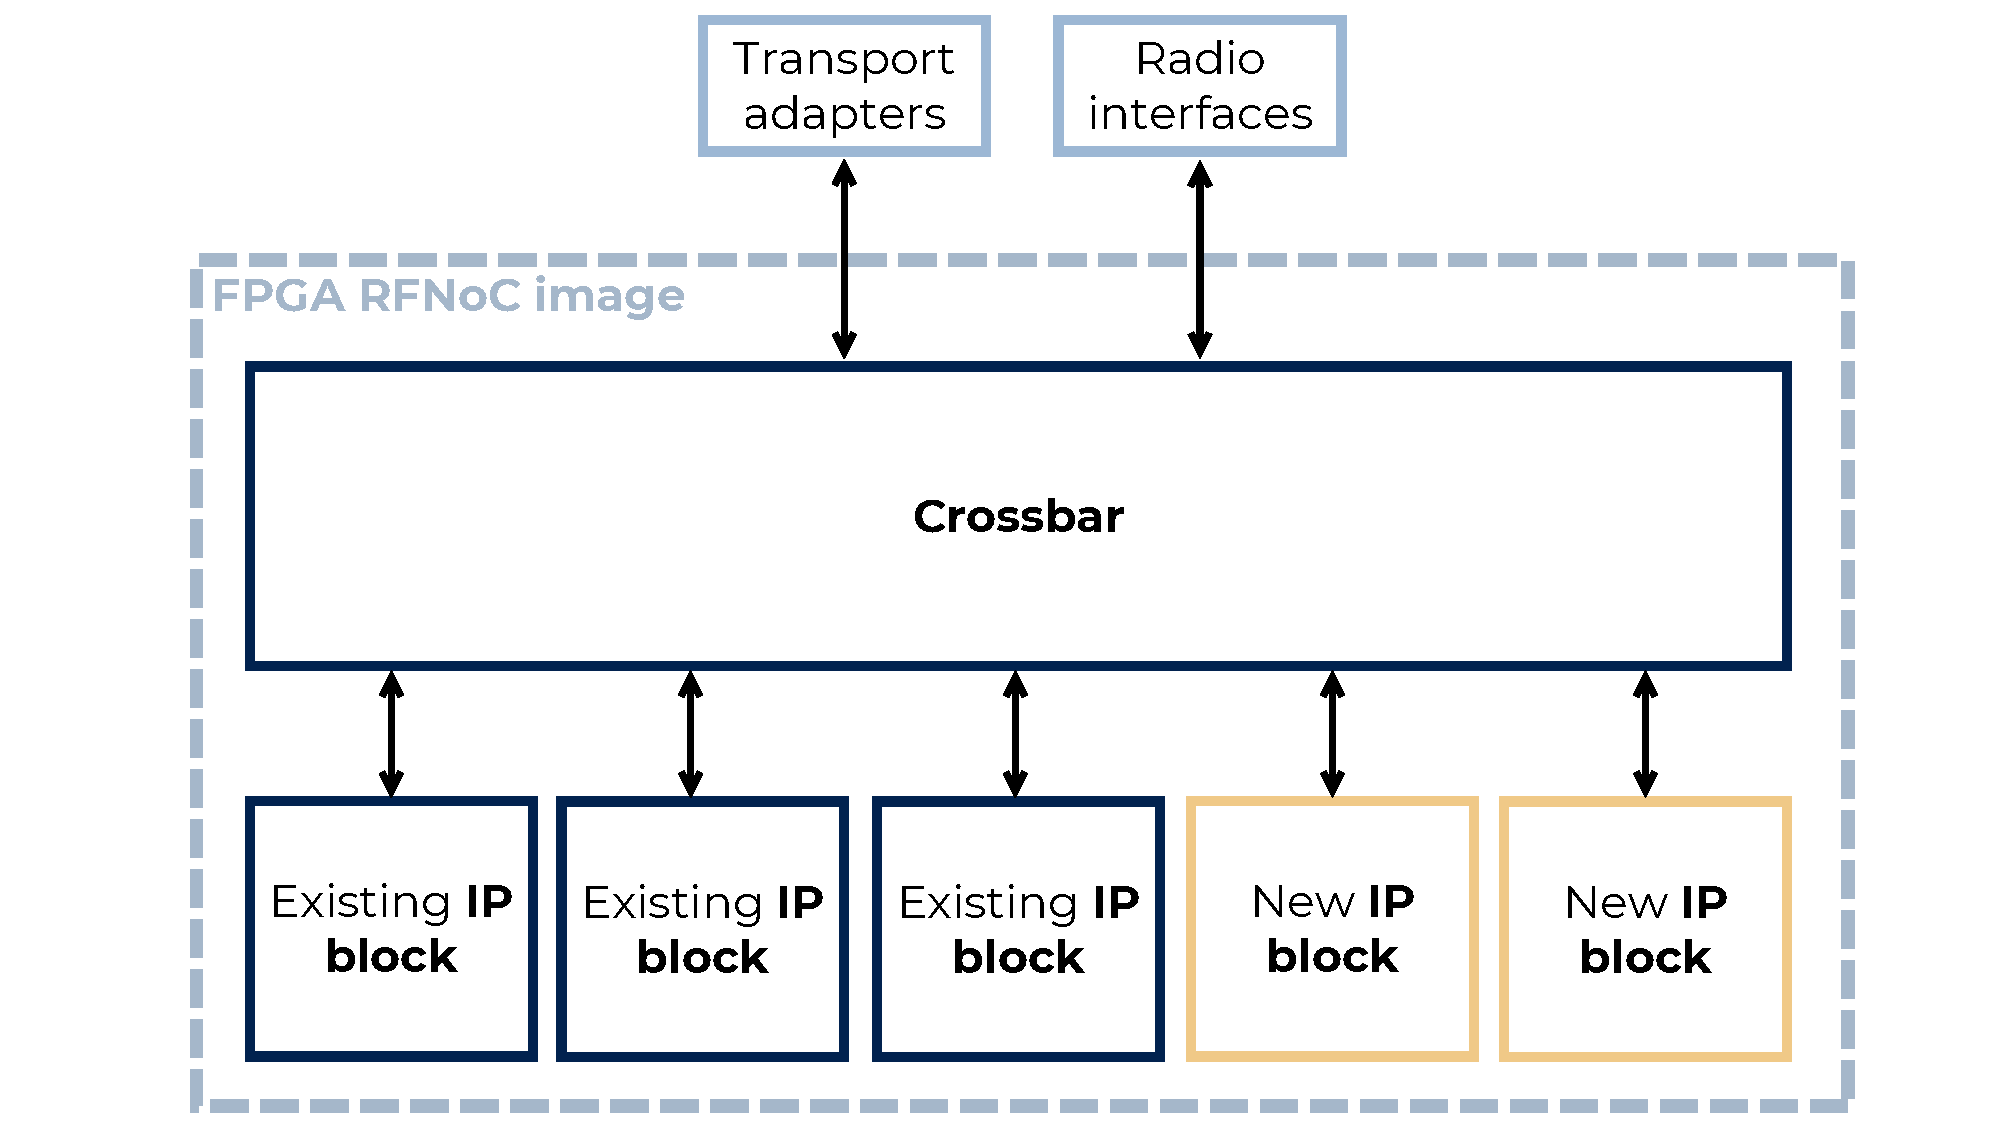
\includegraphics[width=\linewidth]{img/RFNoC.pdf}
      \caption{RFNoC framework vizualisation}
    \end{figure}

  \end{block}
\end{column}


\begin{column}{\sepwid}\end{column} % Empty spacer column

%\begin{block}{Acknowlegdments}
%Here go the acknowledgments.
%\end{block}

\end{columns} % End of all the columns in the poster
\vspace{-1in}
\begin{center}
  \usebeamerfont{block body} Academic year 2024-2025
\end{center}

\end{frame}

\end{document}
